\documentclass[11pt]{article}
\usepackage{amsfonts,amssymb,amsmath,amsthm,amscd}
\usepackage{courier}
\usepackage{mathtools}
\usepackage{fancyhdr}
\usepackage{enumitem}
\usepackage{newtxtext,newtxmath}
\usepackage{listings}
\usepackage{wasysym}
\usepackage{makecell}
\usepackage[linesnumbered,ruled]{algorithm2e}
\usepackage[margin=2.5cm]{geometry}
\parindent 0px

%Header
\fancyhf{}
\setlength{\headheight}{50pt}
\pagestyle{fancy}
\lhead{Matt Uryga\\Yu-Kai Wang\\David Qiu\\Jonathan Li}
\chead{{\bf\LARGE Movie Critic}\\[2mm]Final Report}
\rhead{12/09/2022\\CSCI-4962\\Fall 2022}
\cfoot{\thepage}
\headsep 5mm

%Document
\allowdisplaybreaks

%List set
\lstset{frame=tb, language=python, basicstyle={\small\ttfamily}}

%Functions
\newcommand{\prob}[1]{{\Large\textbf{#1}}}
\newcommand{\npr}{\\[8mm]}
\newcommand{\itm}[1]{\item[(#1)]}
\newcommand{\np}{\newpage}
\newcommand{\N}{\mathbb{N}}
\newcommand{\Z}{\mathbb{Z}}
\newcommand{\Q}{\mathbb{Q}}
\newcommand{\R}{\mathbb{R}}
\newcommand{\C}{\mathbb{C}}
\newcommand{\D}{\mathcal{D}}
\newcommand{\PP}{\mathbb{P}}
\newcommand{\HH}{\mathcal{H}}
\newcommand{\PPT}[1]{\PP(\text{#1})}
\newcommand{\E}{\mathbb{E}}
\newcommand{\ET}[1]{\E[\text{#1}]}
\newcommand{\Lang}{\mathcal{L}}
\newcommand{\pminf}{_{-\infty}^{+\infty}}
\newcommand{\schrodeq}{-\frac{\hslash^2}{2m}\PPartial{\Psi(x,t)}{x}+V(x)\Psi(x,t)=i\hslash\Partial{\Psi(x,t)}{t}}
\newcommand{\st}{^{*}}
\newcommand{\Claim}{{\bf Claim: }}
\newcommand\sbullet[1][1]{\mathbin{\ThisStyle{\vcenter{\hbox{%
	\scalebox{#1}{$\SavedStyle\bullet$}}}}}%
}
\newcommand*\circled[1]{\tikz[baseline=(char.base)]{
						\node[shape=circle,draw,inner sep=1pt] (char) {#1};}}
\newcommand{\hs}{\hslash}
\newcommand{\eiet}[1]{e^{\frac{iE_{#1}t}{\hslash}}}
\newcommand{\neiet}[1]{e^{-\frac{iE_{#1}t}{\hslash}}}
\newcommand{\eikx}[1]{e^{ik_{#1}x}}
\newcommand{\neikx}[1]{e^{-ik_{#1}x}}
\newcommand{\pr}{^\prime}
\newcommand{\ppr}{^{\prime\prime}}
\newcommand{\pppr}{^{\prime\prime\prime}}
\newcommand{\ppppr}{^{\prime\prime\prime\prime}}
\newcommand{\op}[1]{\hat #1}
\newcommand{\dg}{^\dagger}
\newcommand{\lal}{(\alph*)}
\newcommand{\lrom}{(\roman*)}
\newcommand{\lara}{(\arabic*)}
\newcommand{\comm}[2]{\left[\hat{#1},\hat{#2}\right]}
\newcommand{\xyz}{(x,y,z)}
\newcommand{\bbar}[1]{\mkern 1.5mu\overline{\mkern-1.5mu#1\mkern-1.5mu}\mkern 1.5mu}
\newcommand{\dx}{\,dx}
\newcommand{\oneminus}[1]{\left(1-#1\right)}
\newcommand{\hi}{\frac{\hs}{i}}
\newcommand{\ih}{\frac{i}{\hs}}
\newcommand{\e}[1]{\cdot10^{#1}}
\newcommand{\hv}{\inv{2}}
\newcommand{\inv}[1]{\frac{1}{#1}}
\newcommand{\invsq}[1]{\frac{1}{\sqrt{#1}}}
\newcommand{\sqfr}[2]{\sqrt\frac{#1}{#2}}
\newcommand{\Partial}[2]{\frac{\partial #1}{\partial #2}}
\newcommand{\PPartial}[2]{\frac{\partial^2 #1}{\partial #2^2}}
\newcommand{\FPartial}[2]{\frac{\partial}{\partial #2}#1}
\newcommand{\FPPartial}[2]{\frac{\partial^2}{\partial #2^2}#1}
\newcommand{\FpPartial}[2]{\frac{\partial}{\partial #2}\left(#1\right)}
\newcommand{\FpPPartial}[2]{\frac{\partial^2}{\partial #2^2}\left(#1\right)}
\newcommand{\deriv}[2]{\frac{d #1}{d #2}}
\newcommand{\dderiv}[2]{\frac{d^2 #1}{d #2^2}}
\newcommand{\expval}[1]{\left\langle #1 \right\rangle}
\newcommand{\vvatrix}[2]{\paren{\begin{matrix}#1\\#2\end{matrix}}}
\newcommand{\vvvatrix}[3]{\paren{\begin{matrix}#1\\#2\\#3\end{matrix}}}
\newcommand{\vvvvatrix}[4]{\paren{\begin{matrix}#1\\#2\\#3\\#4\end{matrix}}}
\newcommand{\hhatrix}[2]{\paren{\begin{matrix}#1&#2\end{matrix}}}
\newcommand{\hhhatrix}[3]{\paren{\begin{matrix}#1&#2&#3\end{matrix}}}
\newcommand{\hhhhatrix}[4]{\paren{\begin{matrix}#1&#2&#3&#4\end{matrix}}}
\newcommand{\mmatrix}[4]{\paren{\begin{matrix}#1&#2\\#3&#4\end{matrix}}}
\newcommand{\mmmatrix}[9]{\paren{\begin{matrix}#1&#2&#3\\#4&#5&#6\\#7&#8&#9\end{matrix}}}
\newcommand{\ccases}[4]{\begin{cases}#1&#2\\#3&#4\end{cases}}
\newcommand{\norm}[1]{\left|\left|#1\right|\right|}
\newcommand{\paren}[1]{\left(#1\right)}
\newcommand{\eps}{\epsilon}
\newcommand{\magn}[1]{\left|\left|#1\right|\right|}
\newcommand{\bs}[1]{\boldsymbol{#1}}
\newcommand{\mh}{m_{\HH}}
\newcommand{\dvc}{{d_{VC}}}
%Constants
\newcommand{\h}{6.626\e{-34}}
\newcommand{\elec}{1.6\e{-19}}
\newcommand{\elecmass}{9.109\e{-31}}
\newcommand{\cc}{3\e{8}}
%Misc
\DeclarePairedDelimiter\ceil{\lceil}{\rceil}
\DeclarePairedDelimiter\floor{\lfloor}{\rfloor}

\begin{document}
\begin{titlepage}
\begin{center}
	\vspace*{1cm}

	\textbf{\Huge Movie Critic}

	\vspace{0.5cm}
	{\Large Final Report}

	\vspace{1.5cm}

	\textbf{Matt Uryga, Yu-Kai Wang\\David Qiu, Jonathan Li}

	\vfill

	12/09/2022\\
	CSCI-4962\\
	Rensselaer Polytechnic Institute
\end{center}
\end{titlepage}

\setcounter{secnumdepth}{4}
\setcounter{tocdepth}{4}

\tableofcontents
\np

\section{Introduction}
\subsection{Overall Goals}
The primary goal of the project was to construct a model to analyze movie reviews to predict movie ratings.  Sentiment analysis is a crucial part of this - the reviews need to be analyzed through the lens of sentiment analysis to provide accurate and reliable results.


\subsection{Background Information}
For any given movie, there are a plethora of reviews and ratings online.  Bad numerical ratings (less than 5/10) are typically associated with negative reviews, and vice versa.  We hope to be able to predict the numerical value of the rating from the review text.

\subsection{Source Code}
All code and images can be access via https://github.com/DiscreteDigitalDevelopers/Movie-Critic.


\section{Data}
\subsection{Scraping IMDB}
To train our model we need a source of data that is both representational of the population and credible. After some research we chose IMDB to be our main source of data collection.  In this project we will be focusing on sentiment analysis on textual information.  We will be primarily collecting the top 5 reviews for each movie titles and their associated average ratings as the label of our sentiment analysis.
\\[2mm]
IMDB has a public dataset available for all current titles they have in their database, but reviews are not included.  For the purpose of this project, we have developed a web scraper that extracts and download the top reviews of a title given the movie id, which comes with the public dataset released by IMDB.


\subsection{Exploratory Data Analysis}
\subsubsection{Shape of Dataset}
For the ease of training and loading, the final data structure we want to store our data in is a single python dictionary, with keys being the title id, and the values being a tuple of average rating with the top 5 reviews concatenated as single string.  The dictionary will then be stored as a pickle file for later use.

\subsubsection{Train, Validation, Test Splits}
One bottleneck we have encountered during the scraping phase is the internet bandwidth -- we are scraping about 2 titles per seconds, which will take us more than a week to fully scrape all the titles.  Fortunately, judging by the computing power we currently have, our model will not be able to handle the enormous amount of data anyway.  We eventually decided to settle on  28000 titles in total.  This down sampling of the data are randomly generated.  The dataset is than split to training, validation, and testing datasets with sizes of 24000, 2000, and 2000 respectively.
\np

\subsubsection{Distribution of Ratings}
To ensure all the dataset are representational of the entire population, we plotted the ratings distribution diagram below.\\[2mm]
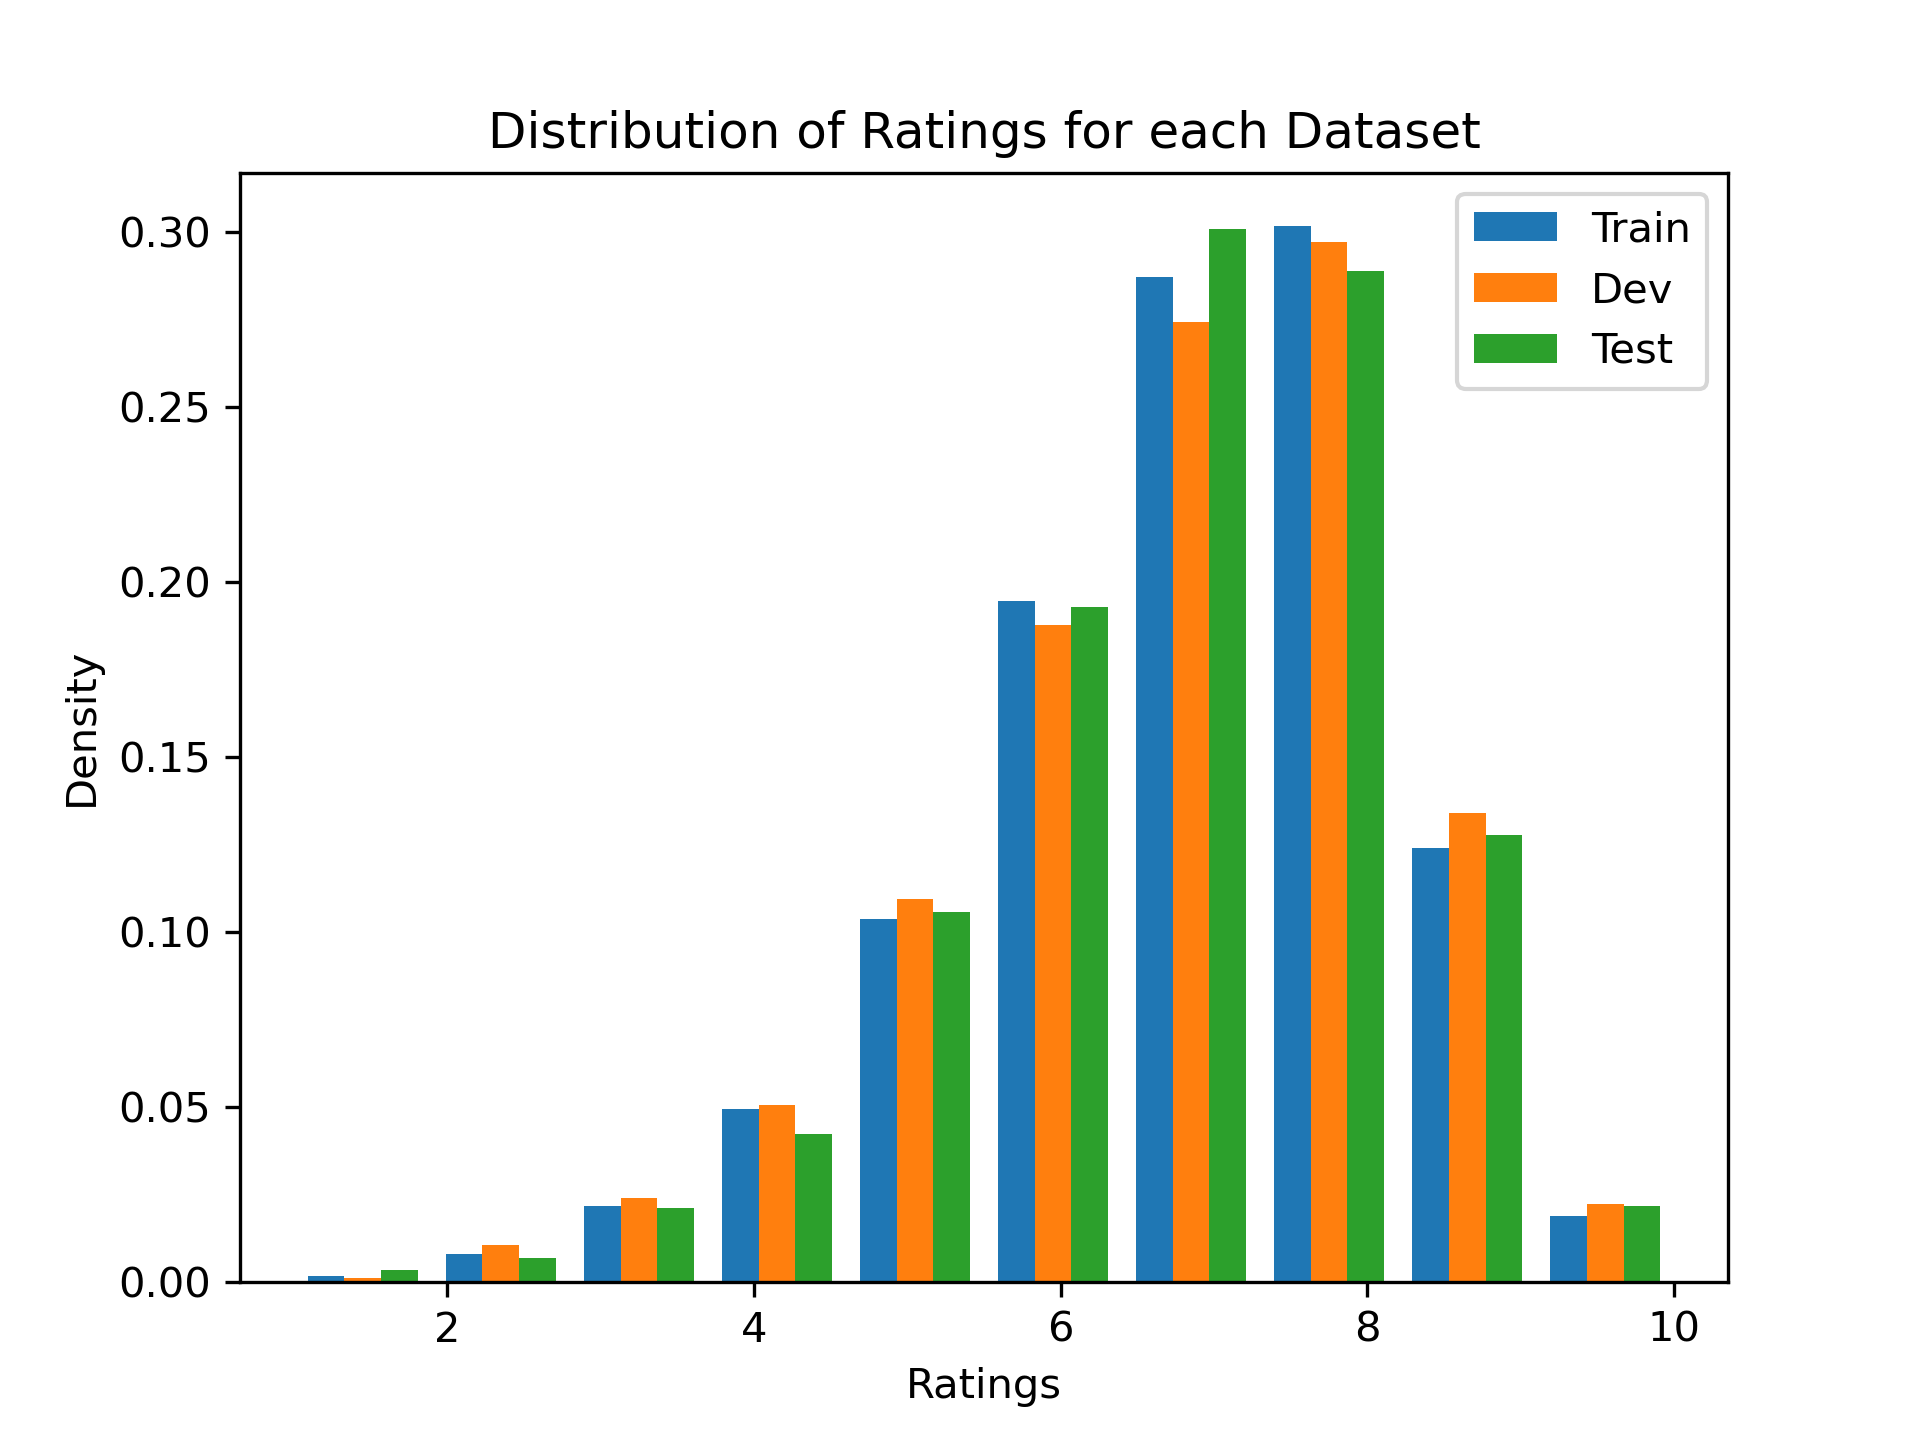
\includegraphics[scale=1]{data_split_distributions.png}\\[2mm]

As we can see, the distribution of the ratings are homogeneous across the train/validation/test split, and is left skewed.  Most of the titles have ratings around 7 to 8, and there are barely any data points with ratings less than 4 or above 9.  This will be a problem for our model as an imbalanced data will introduce unnecessary bias into the model.  Data augmentation is out of question since it is very hard to generate synthetic data for movie reviews.  We will be implementing different weightings for the loss functions depending on the frequency of the ratings instead.
\np



\section{Models}
\subsection{Random Forest}
\subsubsection{Selection of Model}
Random forest was chosen due to its versatility, allowing for us to easily switch between a continuous regression and a ten label classification test if we choose to threshold our labels.  Since movie ratings do not have set thresholds, we decided to use random forest regressor to predict a continuous set of ratings.  Random forest also provides the additional convenience of allowing us to easily see the relative importance of the features in the data provided to it.  We also trained and tested on a gradient boosting model.

\subsubsection{Data Preprocessing}\label{data_processing}
For both our random forest and logistic regression models, our data was preprocessed in the same way.  The data we collected was stored in the form of a dictionary mapping a movie index to a tuple of rating and reviews - a concatenated string of 5 reviews randomly selected and stored as a string.  We parsed the review string by removing HTML tags and non alphabetical terms followed by stop word extraction to remove irrelevant information.  The resulting words were then stemmed - a process to obtain the base form of words to reduce word density.
\\[2mm]
With the preprocessed words, we learned a word embedding and formed our train, test, and validation datasets through taking the mean representation of each word in the review sentence of each movie, giving us a numerical representation of our reviews for each movie.

\subsubsection{Model Architecture}
For our random forest, we used scikit-learn's pre-implemented \texttt{RandomForestRegressor} and\\\texttt{GradientBoostingRegressor}.  The random forest model involves training a set of decision trees and the results from each decision tree is tallied at the end in a voting phase, where the most voted prediction is the prediction of the random forest.  The gradient boosting model takes an alternative approach where a sequence of decision trees are trained off of the error from the previous tree.  Like the random forest model, there is also a voting period at the end where the prediction with the most votes will be the output.
\\[2mm]
We supplied our own number of estimators (50), min sample split (3), and max depth (10).  Overall, our model had a mean squared error of 0.74 on the training set and 1.33 on the testing set.  Upon plotting our prediction distribution, we see that both the \texttt{GradientBoostingRegressor} and \texttt{RandomForestRegressor} prioritize the labels 6 and 7, which through our data scraping we learned is where most of the ratings are distributed.  We also thresholded the continuous predictions to obtain a general idea of the accuracy, which was about 74\% for training and 69\% for testing.  We believe that the accuracy will drastically increase if we have a more even distribution of ratings in the training set, which will generalize better.
\np

\subsection{Logistic Regression}
\subsubsection{Selection of Model}
Logistic regression is a staple method of regression and predicting continuous values.  We chose this model as a good baseline model to compare other models to.  Another benefit of logistic regression is it's ability to handle outliers in data, which our dataset has a fair amount of.  Hence, we have chosen logistic regression as one of our models.

\subsubsection{Data Preprocessing}
See \ref{data_processing}.

\subsubsection{Model Architecture}
For our logistic regression model, we use the pre-implemented \texttt{LogisticRegression} from scikit-learn.  The logistic regression model builds a regression model that attempts to predict the probability that a data entry belongs to a certain category, modeled using the sigmoid function.  The scikit-learn implementation of logistic regression allows us to weigh the weights of the input classes if provided, which we utilized to balance out the distribution of our input data which we know are around the 6-8 range.  We see that our model predicts a broader range of values, but at the cost of accuracy on the ten class problem, with an accuracy of 65\% for the testing set.  Our final loss for the regression problem was 4.4 using mean squared error.


\subsection{BERT}
\subsubsection{Selection of Model}
Bidirectional Encoder Representations from Transformers (BERT) is a transformer-based model that is specifically designed for natural language (NLP) processing.  It is a state-of-the-art model for NLP and is utilized heavily in a variety of tasks; Google, for instance, is using BERT in nearly every English query.  BERT can take an extremely large amount of resources to effectively train, however, it is common to import a pre-trained BERT model and fine tune it on a specific dataset.

\subsubsection{Data Preprocessing}
\paragraph{Window and Stride}\mbox{}\\[2mm]
The 24,000 training reviews have a large variation in length, and to standardize the review length, the model was trained on 256 word chunks.  If a review was not long enough, padding and a mask was added to account for the lack of data.  For longer reviews, the model would look at words 0 to 255, and then 32 to 287, and so on until the end of the review was reached.  This helps augment the dataset and it provides much needed additional data to train on.

\paragraph{Tokenization}\mbox{}\\[2mm]
BERT requires specific data in a specific format; as such, it is necessary to tokenize the words that are going to be sent to the model.  This was done through the \texttt{transformers} package that provides a tokenizer for BERT (\texttt{BertTokenizer}).  The tokenizer encodes the data into several arrays containing ids, an attention mask, and other various information needed for the model.

\paragraph{Performance Considerations}\mbox{}\\[2mm]
Tokenizing is resource heavy, and as such, the train, validation, and test datasets were tokenized and saved to a \texttt{pickle} file for quick loading.  This reduced training time significantly.

\subsubsection{Model Architecture}
BERT is composed of a number of repeating encoder blocks that are then fed into a feed forward network.  Each encoder block consists of a multi-head attention module, followed by normalization with residuals.  This is then fed into a feed forward network, and again normalized with residuals.  The number of consecutive encoder blocks is dependent on the size of the model - common choices are 12 and 24.\\[2mm]
The model used for this assignment was a pre-trained BERT model.  Training a BERT model from scratch is not feasible given the resources and time that it requires.  The model was, however, fine tuned on the IMDB reviews.  The results from the BERT model were fed into a small feed forward network that reduced the outputs to one.

\subsubsection{Loss}
The loss function used was mean squared error (MSE).  For this particular regression task, it was decided that MSE would be the most effective.  It penalizes bad predictions heavily which is desirable given the scarcity of bad reviews in the dataset.
\np


\section{Results}
\subsection{Random Forest}
\subsubsection{Scatter Distribution and Histogram}
\mbox{}\\
\begin{minipage}{0.45\textwidth}
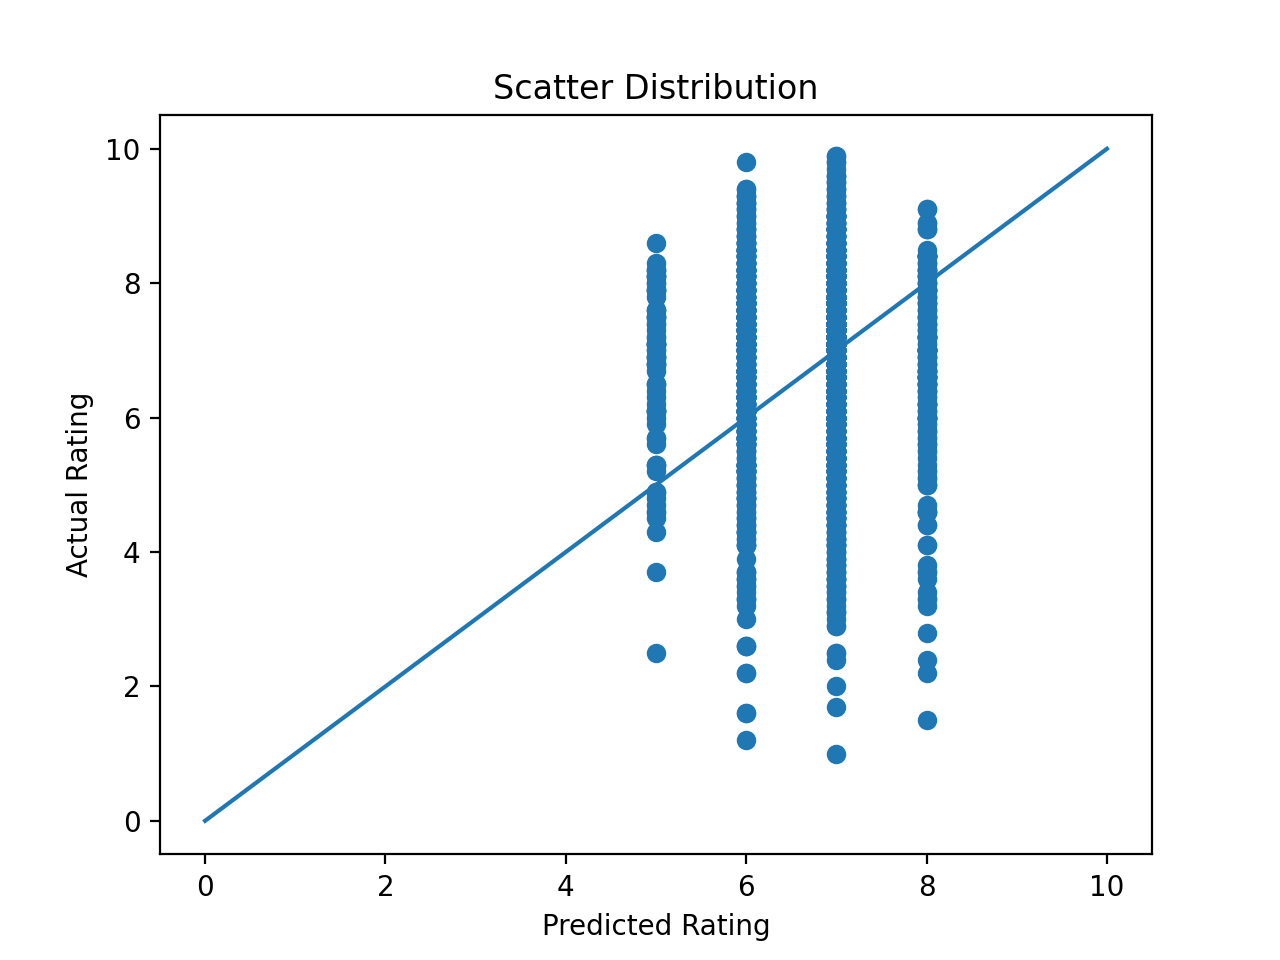
\includegraphics[scale=0.5]{random_forest/scatter.png}
\end{minipage}
\hfill
\begin{minipage}{0.45\textwidth}
\mbox{}\\
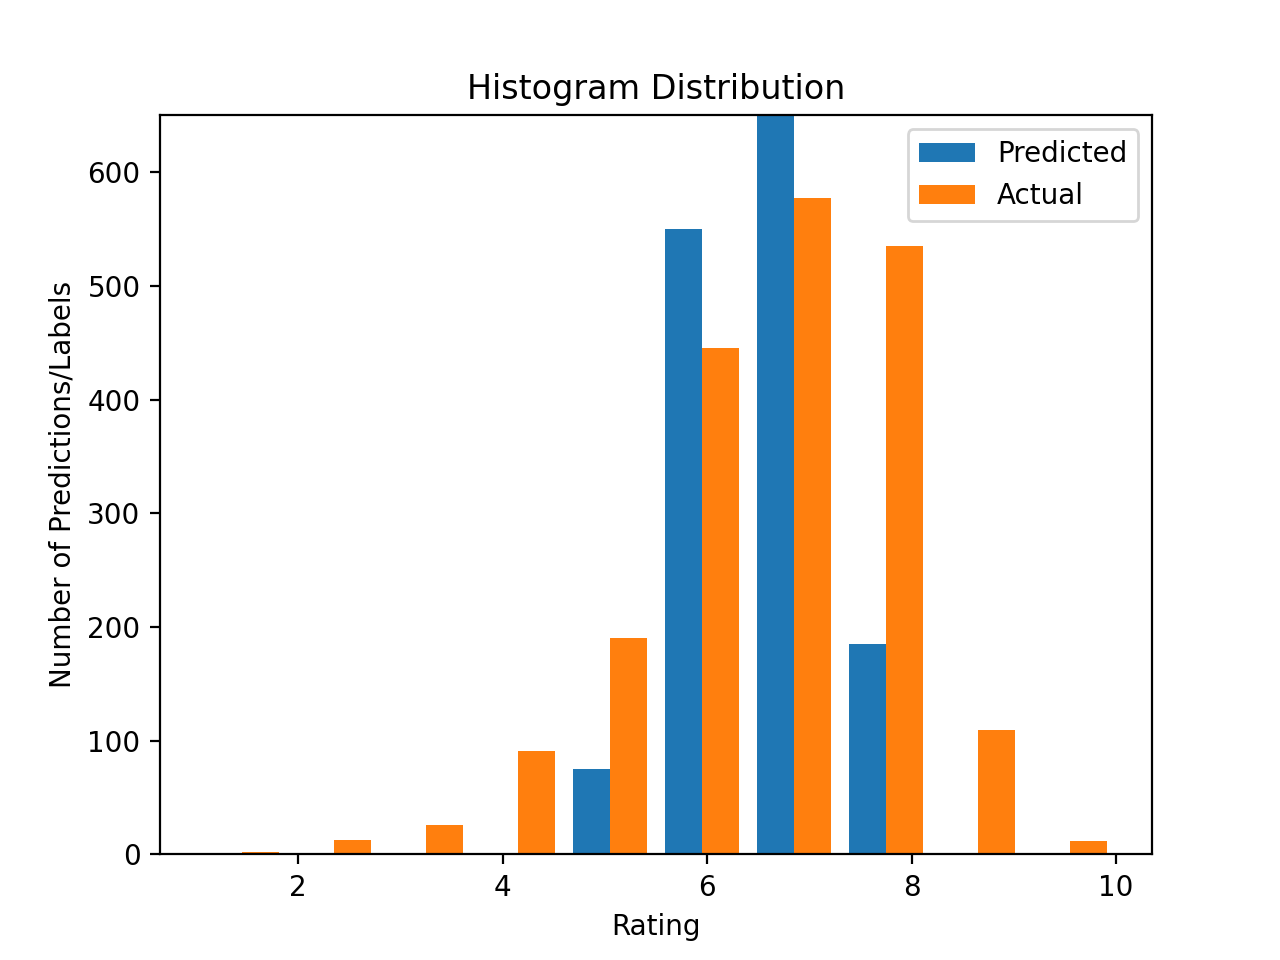
\includegraphics[scale=0.5]{random_forest/histogram.png}
\end{minipage}

\subsubsection{Error Distributions}
\mbox{}\\
\begin{minipage}{0.45\textwidth}
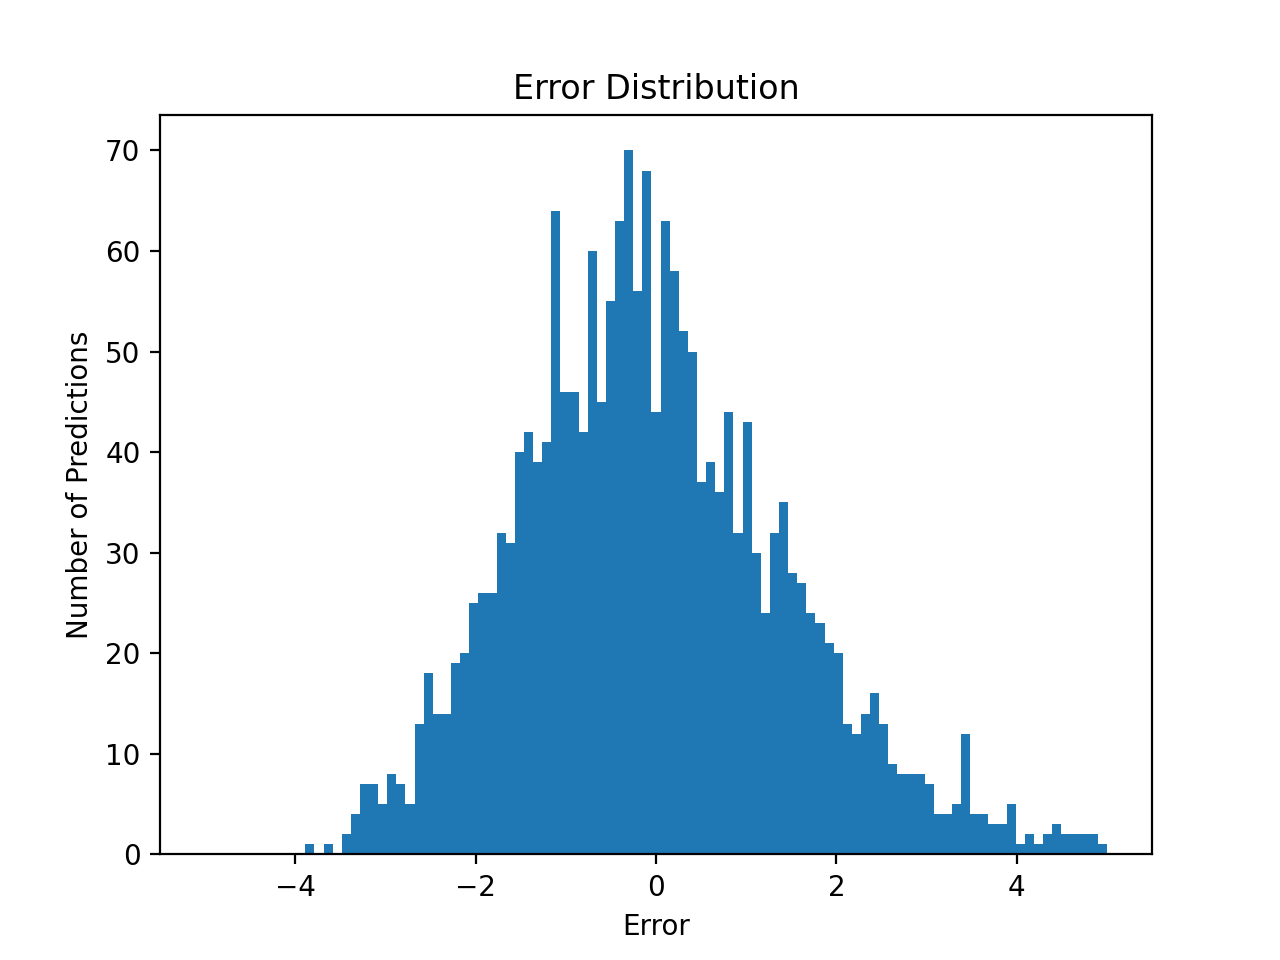
\includegraphics[scale=0.5]{random_forest/error.png}
\end{minipage}
\hfill
\begin{minipage}{0.45\textwidth}
\mbox{}\\
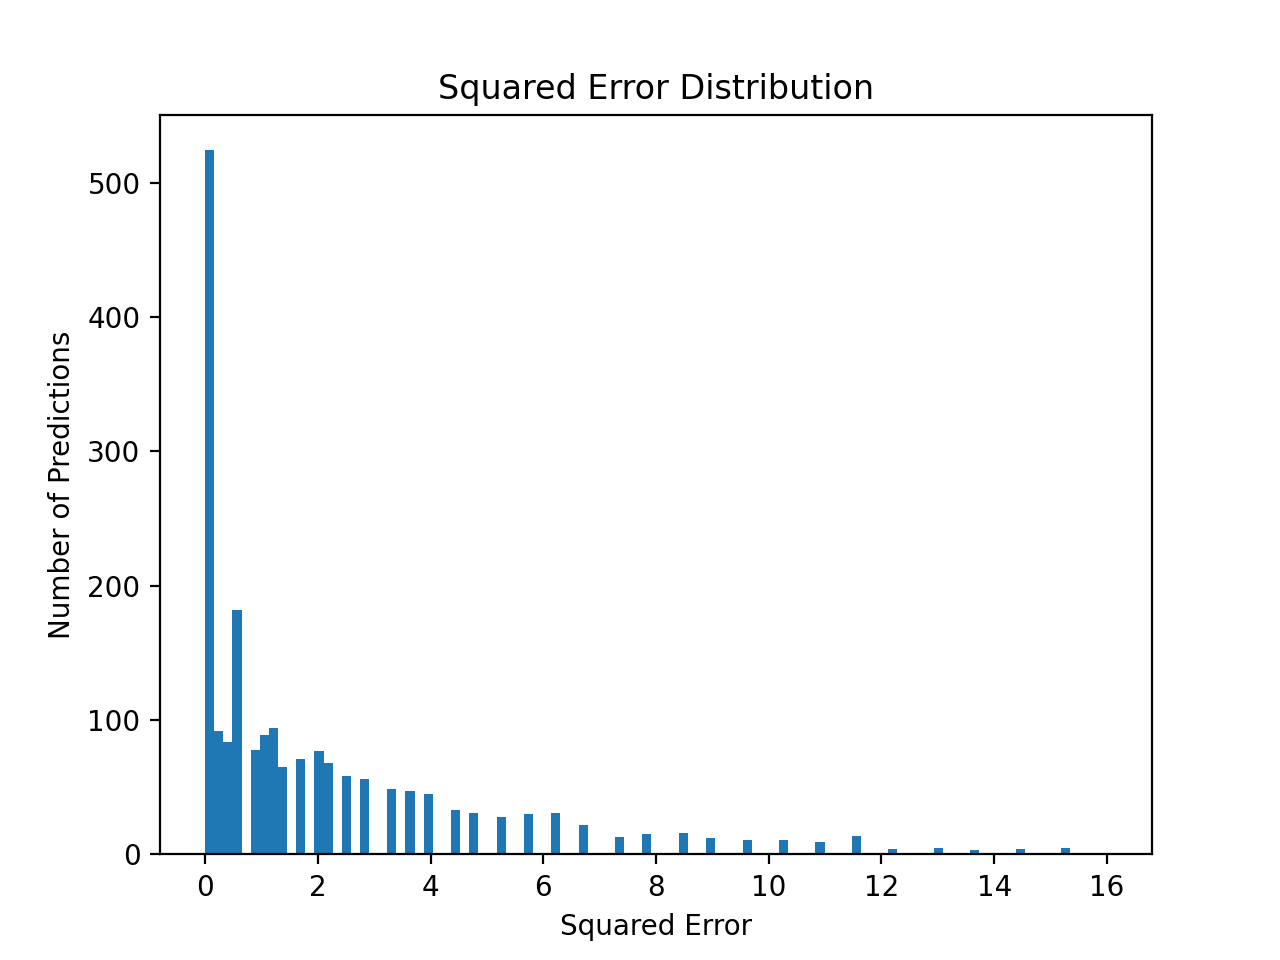
\includegraphics[scale=0.5]{random_forest/squared_error.png}
\end{minipage}


\subsection{Logistic Regression}
\subsubsection{Scatter Distribution and Histogram}
\mbox{}\\
\begin{minipage}{0.45\textwidth}
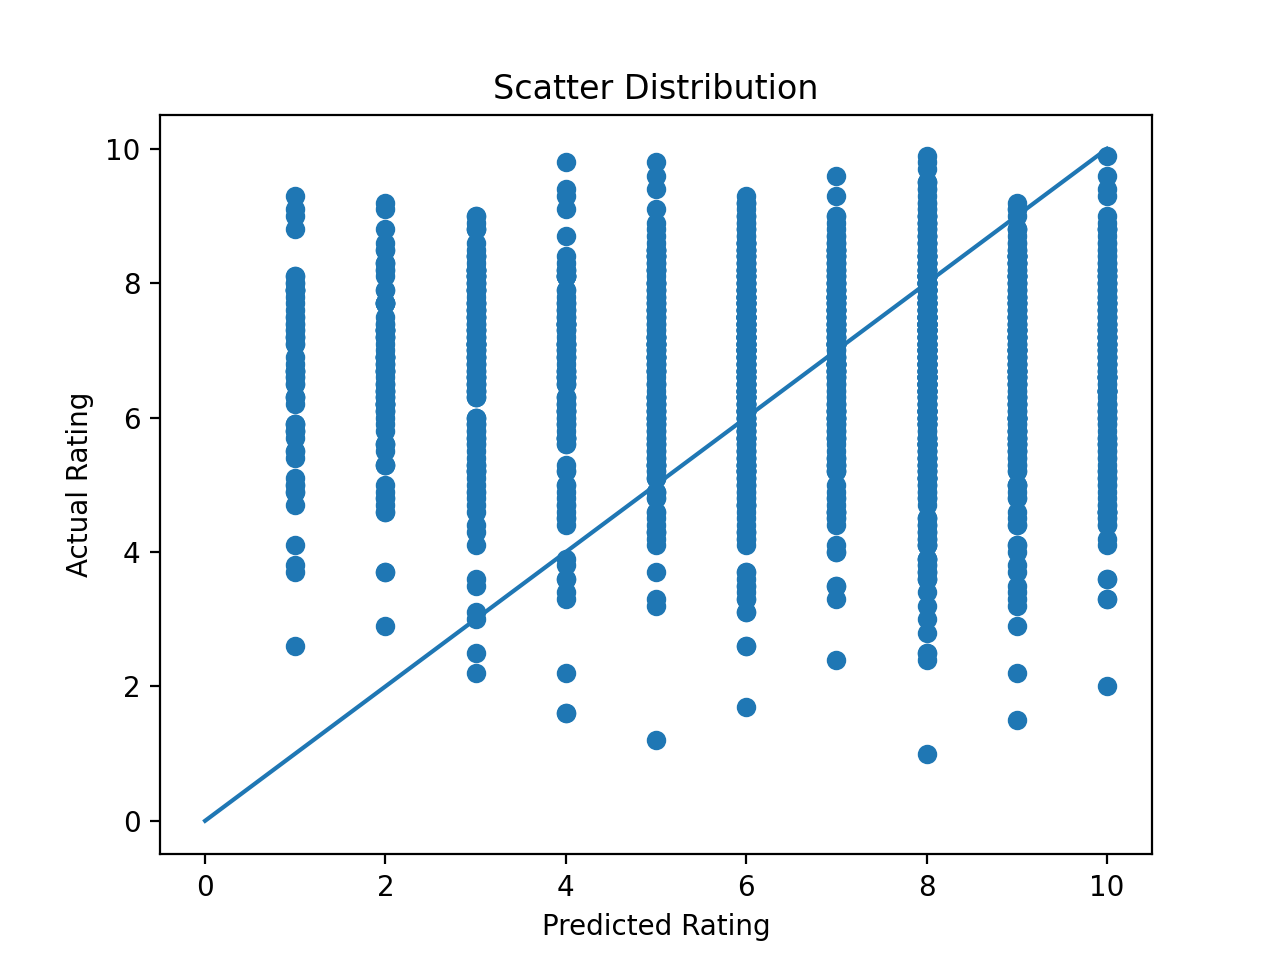
\includegraphics[scale=0.5]{logistic_regression/scatter.png}
\end{minipage}
\hfill
\begin{minipage}{0.45\textwidth}
\mbox{}\\
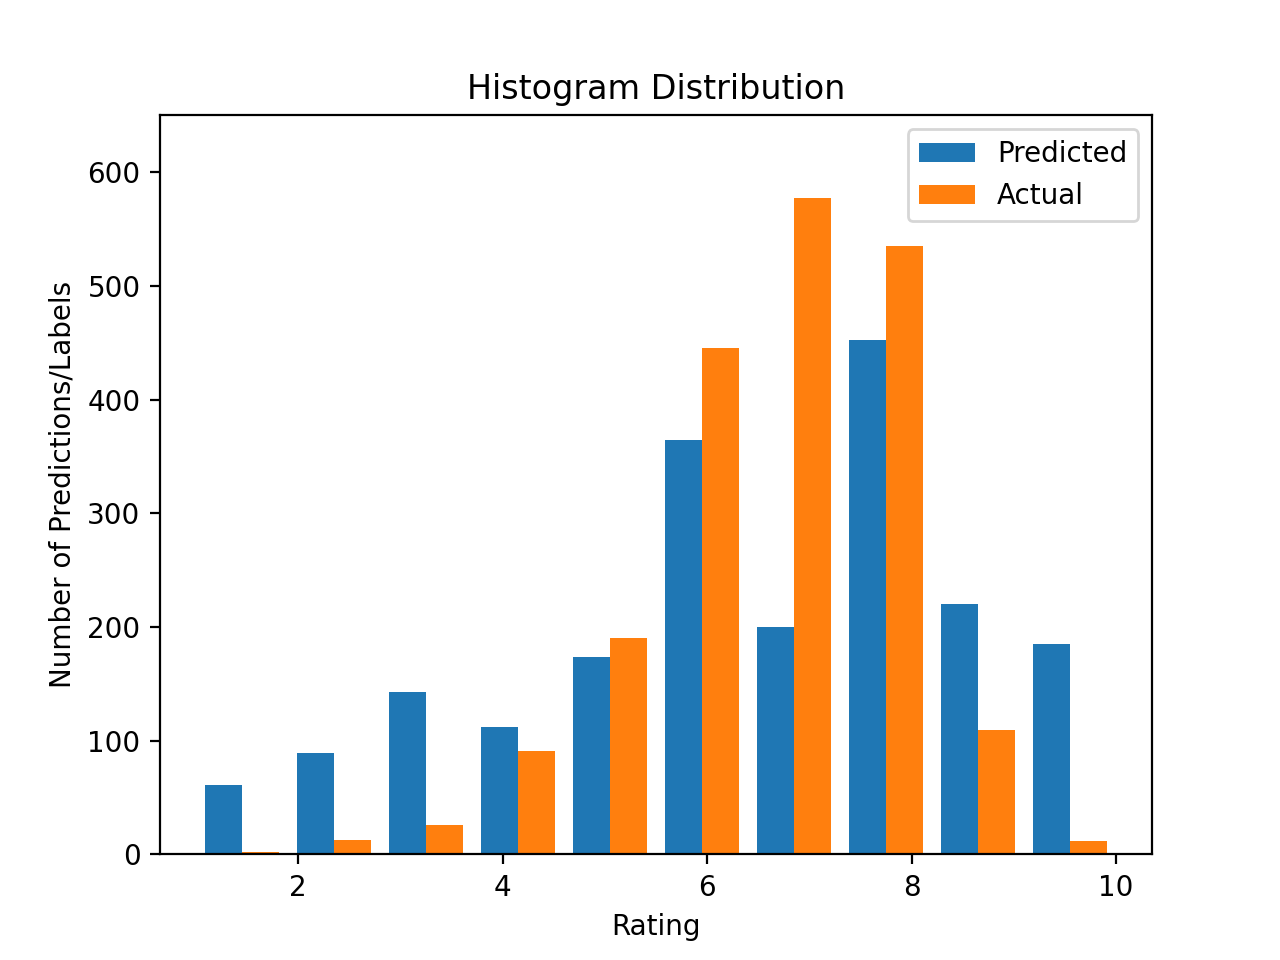
\includegraphics[scale=0.5]{logistic_regression/histogram.png}
\end{minipage}

\subsubsection{Error Distributions}
\mbox{}\\
\begin{minipage}{0.45\textwidth}
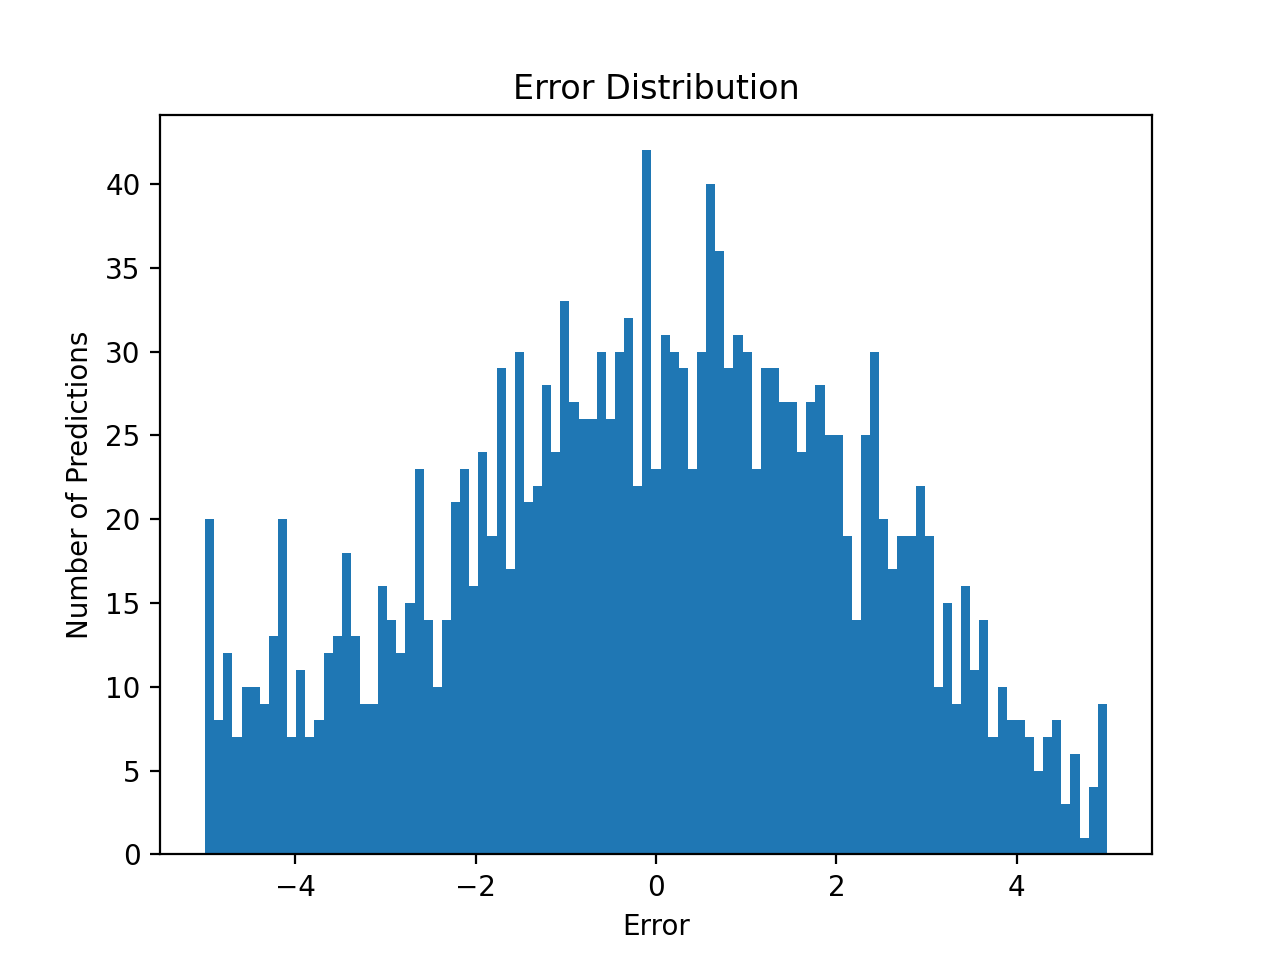
\includegraphics[scale=0.5]{logistic_regression/error.png}
\end{minipage}
\hfill
\begin{minipage}{0.45\textwidth}
\mbox{}\\
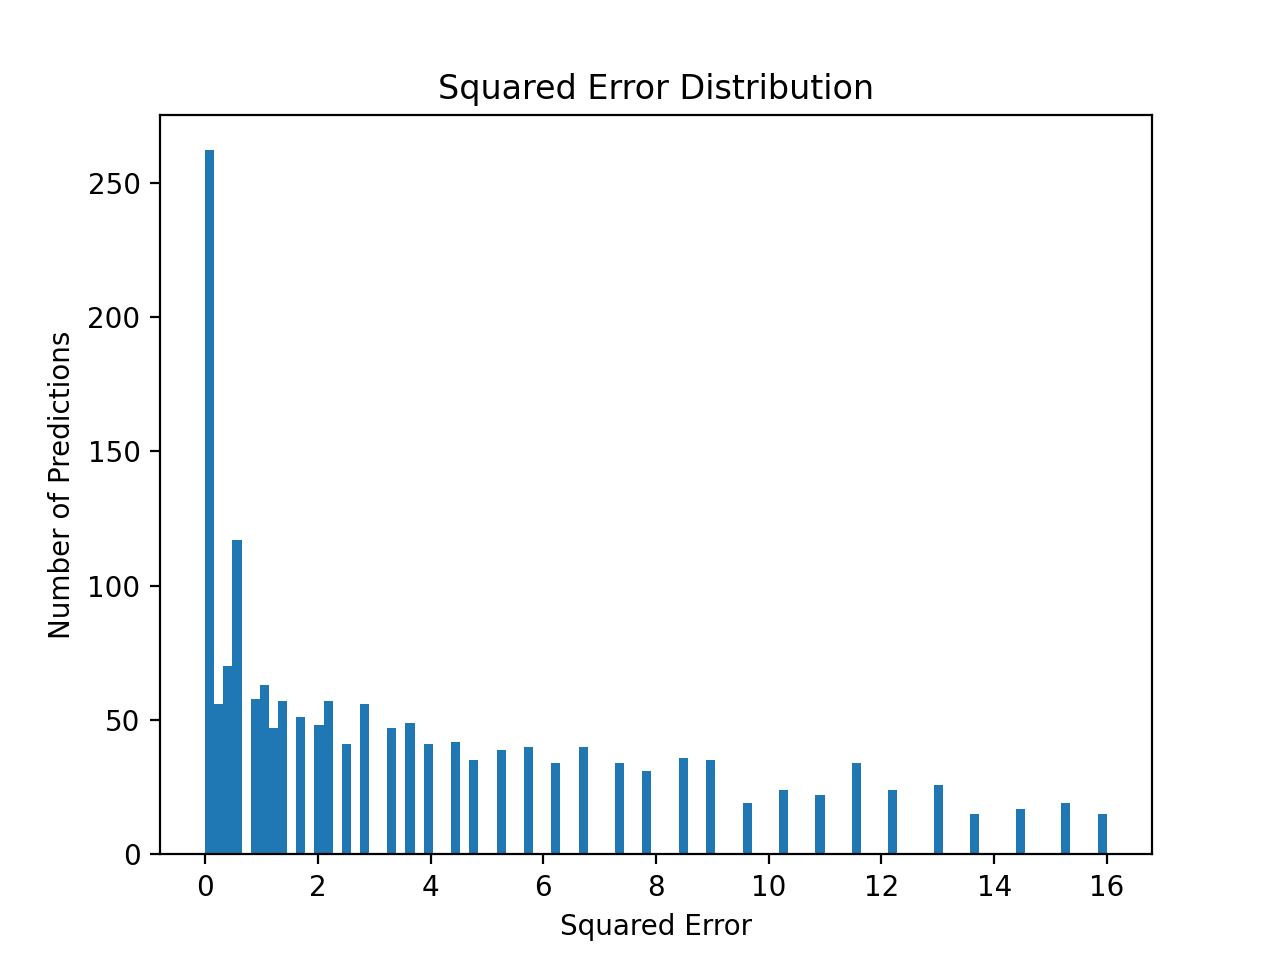
\includegraphics[scale=0.5]{logistic_regression/squared_error.png}
\end{minipage}


\subsection{BERT}
\subsubsection{Scatter Distribution and Histogram}
\mbox{}\\
\begin{minipage}{0.45\textwidth}
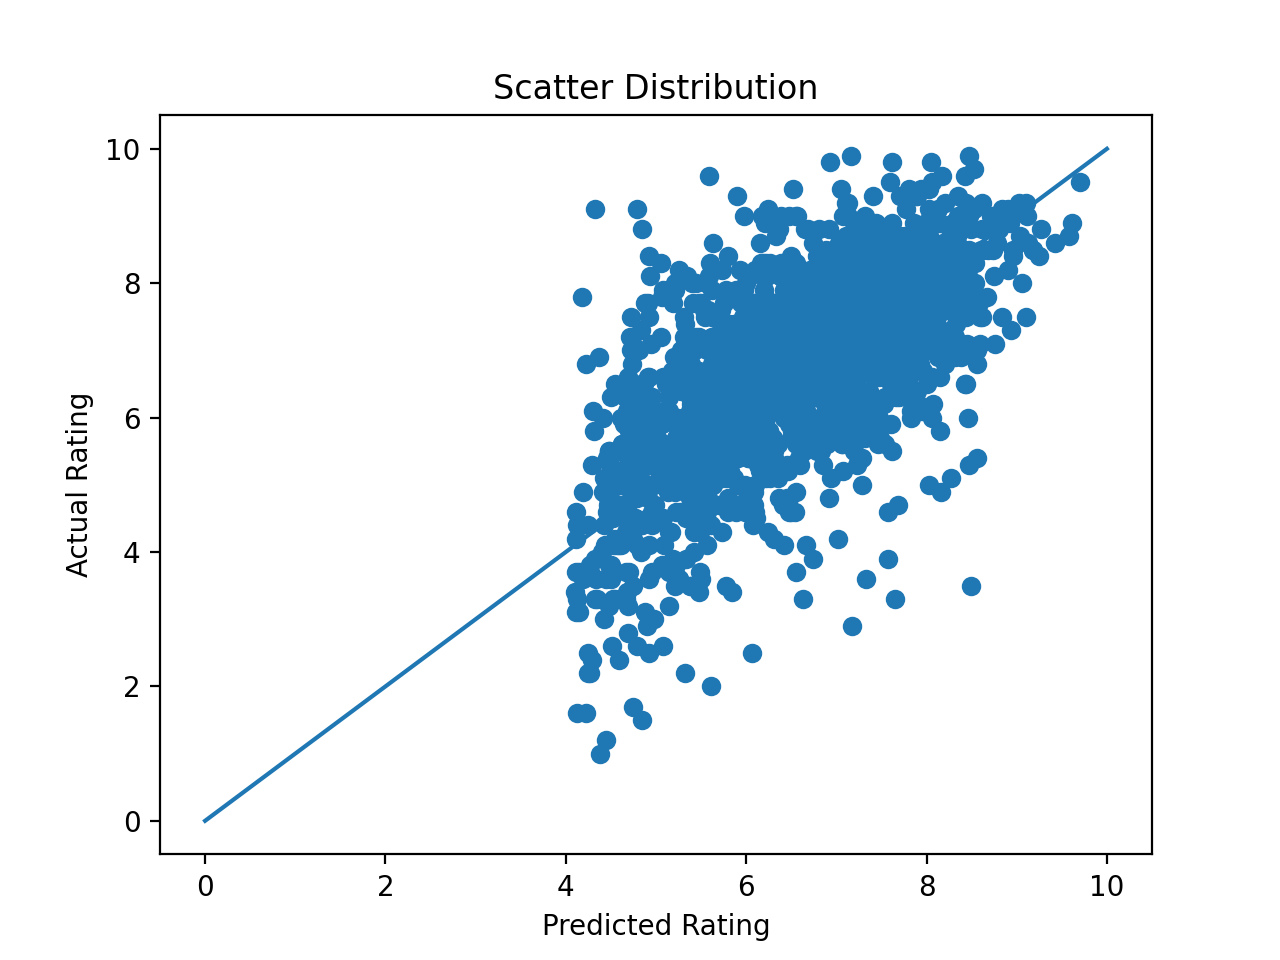
\includegraphics[scale=0.5]{bert/scatter.png}
\end{minipage}
\hfill
\begin{minipage}{0.45\textwidth}
\mbox{}\\
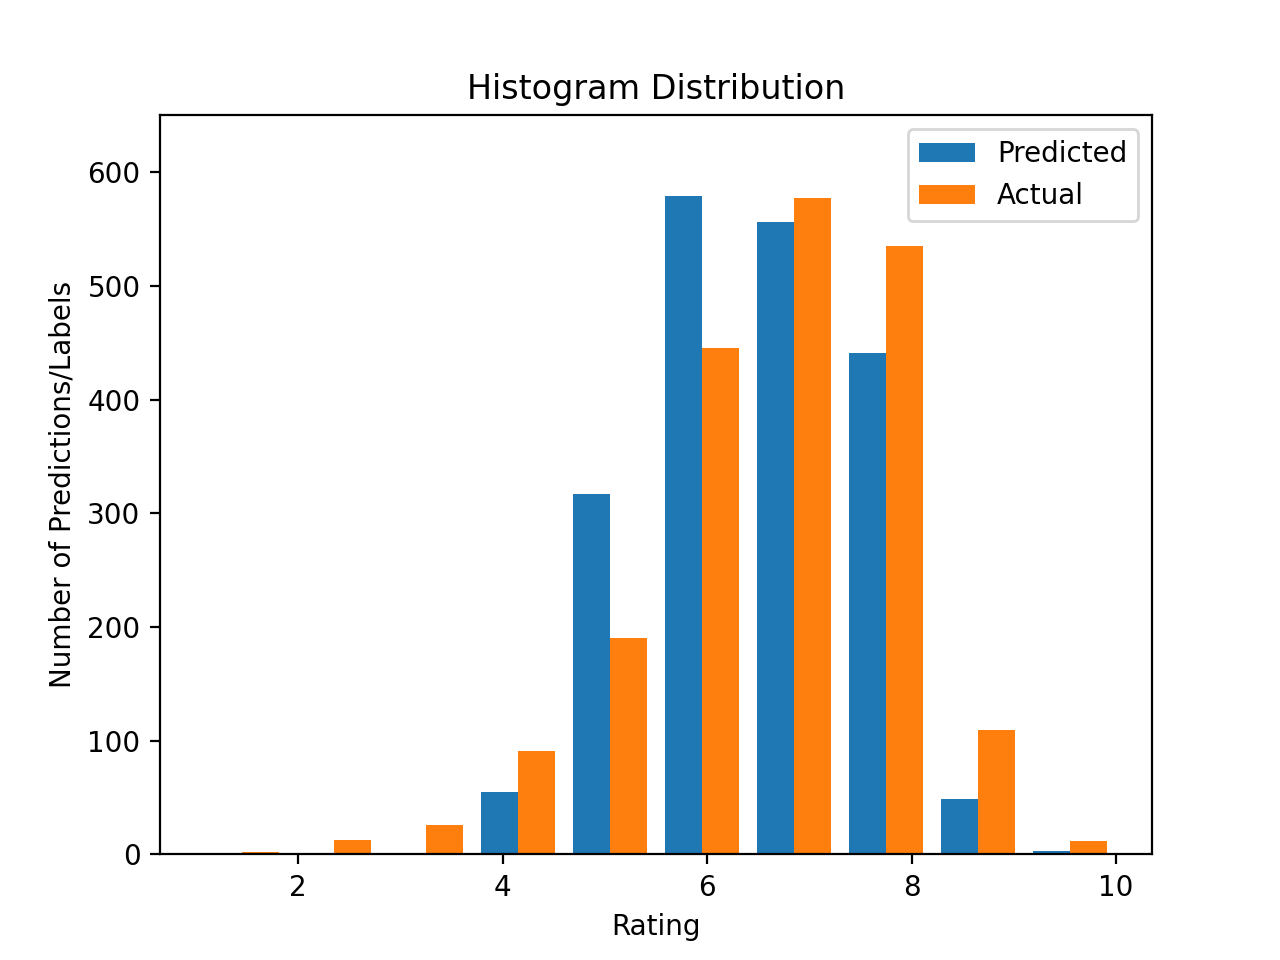
\includegraphics[scale=0.5]{bert/histogram.png}
\end{minipage}

\subsubsection{Error Distributions}
\mbox{}\\
\begin{minipage}{0.45\textwidth}
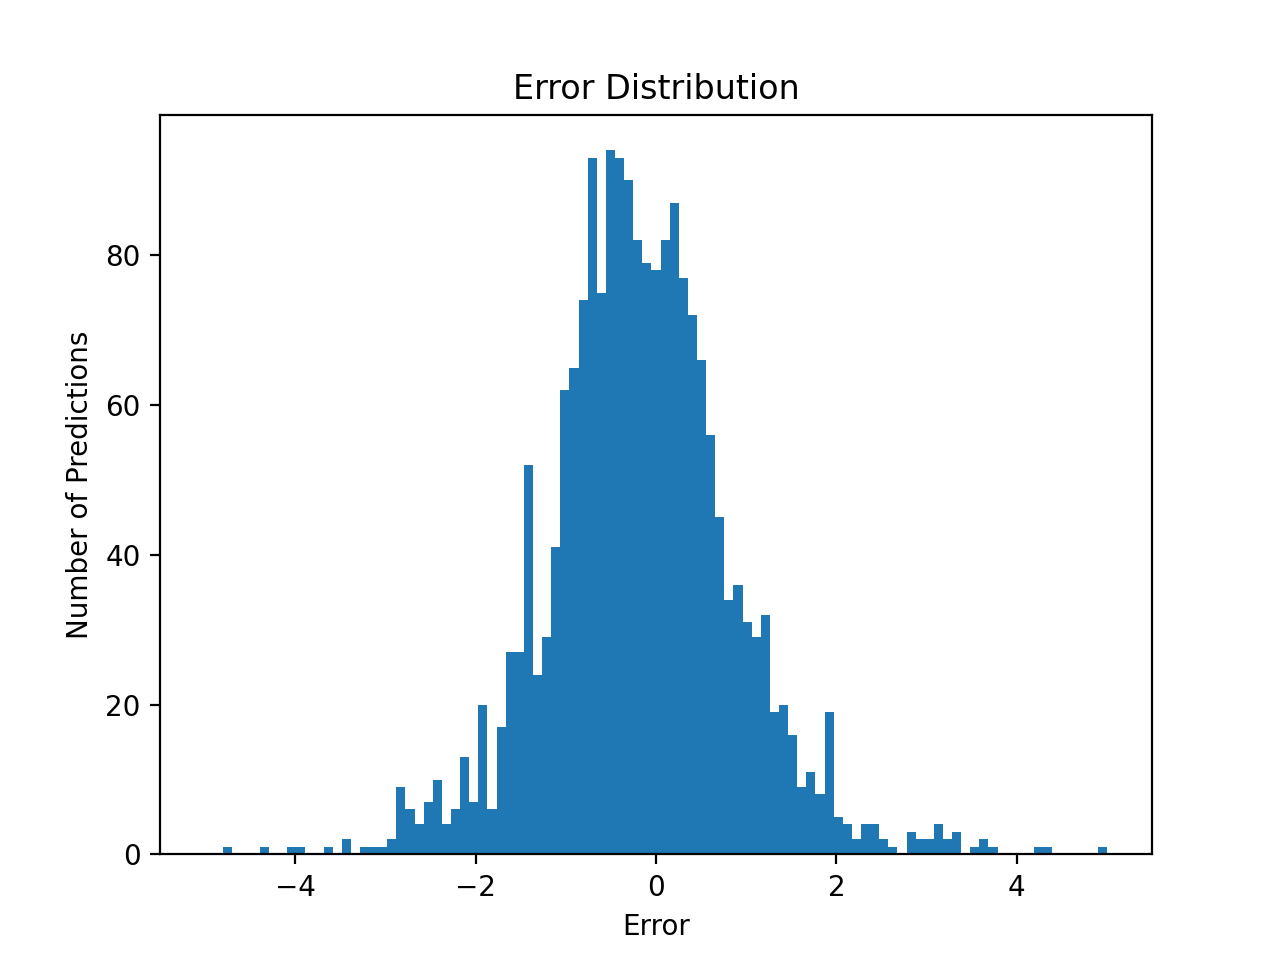
\includegraphics[scale=0.5]{bert/error.png}
\end{minipage}
\hfill
\begin{minipage}{0.45\textwidth}
\mbox{}\\
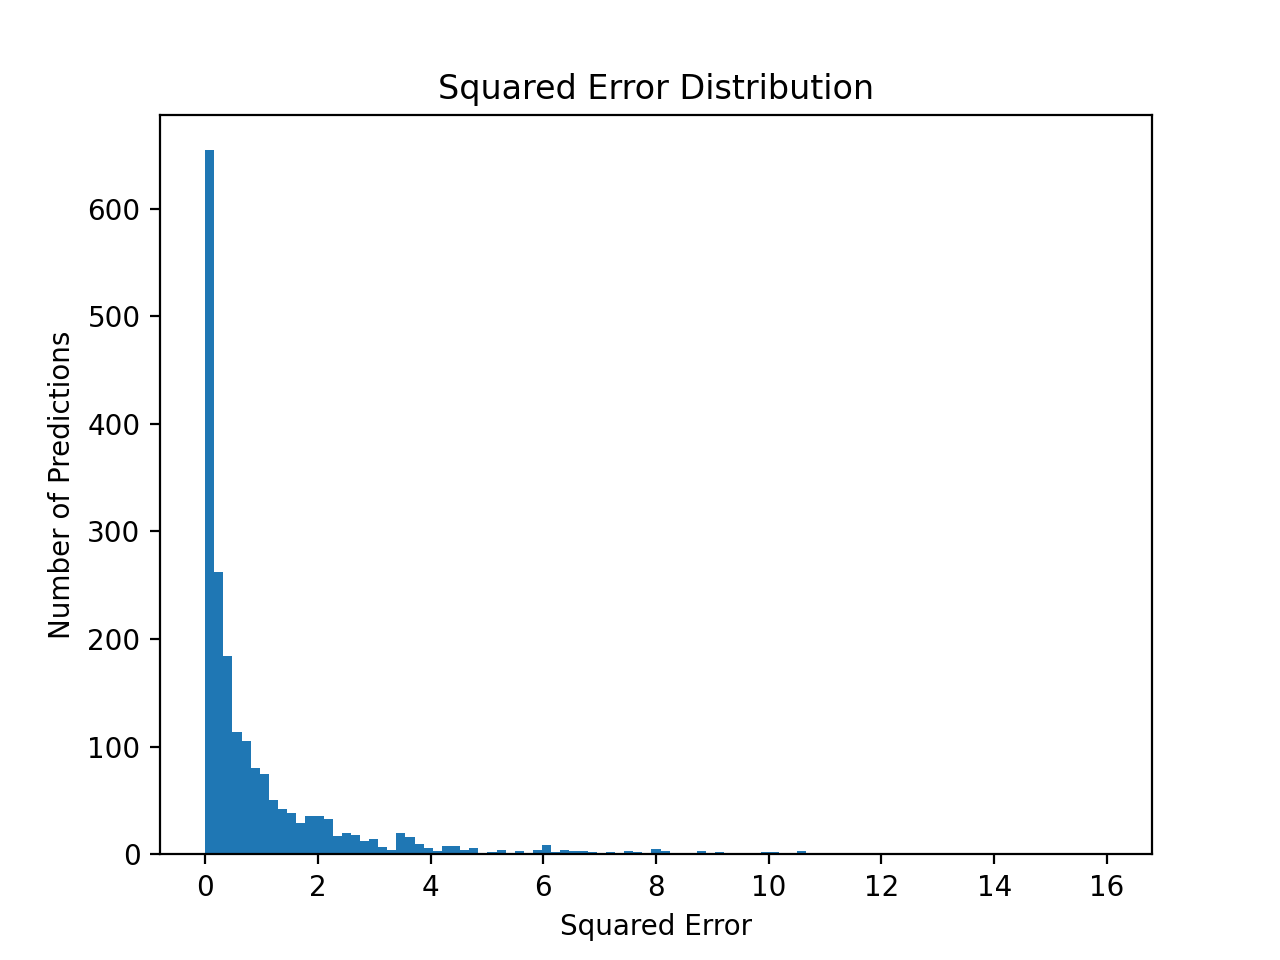
\includegraphics[scale=0.5]{bert/squared_error.png}
\end{minipage}
\np

\subsection{Error Statistics}
\begin{tabular}{c|cccc}
Model & Mean Error & MSE & Std. Dev. of Error & Range of Error\\
\hline
Random Forest & $1.1778$ & $2.2660$ & $1.5053$ & $-3.8000$ to $6.5000$\\
Logistic Regression & $2.1565$ & $7.3299$ & $2.6959$ & $-8.3000$ to $8.000$\\
BERT & $0.8033$ & $1.1179$ & $1.0480$ & $-4.7709$ to $4.9968$
\end{tabular}\\[5mm]
From the results above, it is evident that BERT performs the best out of the 3 models that were trained - by all metrics, it is more accurate and has less variance in the error than the other models.  That being said, the BERT model does not predict any ratings below approximately $4.0$.  This is most likely due to the insufficient number of data points for ratings under $4.0$.
\end{document}